\section{Einleitung}

\subsection{Motivation und Problemstellung}
In der heutigen Zeit erweist sich Flexibilität als eine immer bedeutendere Determinante für den Erfolg von Unternehmen. So müssen diese stets in der Lage sein, sich effizient an verändernde Marktbedingungen anzupassen. Unternehmen sehen sich deshalb vornhemlich damit konfrontiert, die in Enterprise-Ressource-Planning-Systemen (\acs{ERP}-Systemen) abgebildeten Prozesse auf externe Einflüsse, wie Kundenbedürnisse, rechtliche Vorschriften und neue Technologien auszurichten. Mit der \textit{Composable-Enterprise-Architektur (CEA)} hat sich in den vergangenen Jahren ein Konzept etabliert, welches Unternehmen bei der Bewältigung dieser Disruptionen unterstützen soll. In einer CEA werden modulare Software-Komponenten zu einem homogenen Gesamtsystem konsolidiert \cite{.20230313}. Martin Henning, Head of New Ventures and Technologies bei der SAP, bemerkt, dass Unternehmen mit diesem Architekturkonzept nicht länger auf \enquote{rigide Systeme} angewiesen, sondern vielmehr in der Lage sind, Geschäftsprozesse auf Grundlage einzelner Software-Bausteine zusammenzusetzen \cite{Galer.20221019}. Bei einer Änderung der Geschäftsanforderungen besteht somit die Möglichkeit einzelne Software-Komponenten dynamisch auzutauschen ohne, dass Anpassungen am Gesamtsystem erforderlich sind. Dieser Composable-Trend ist nicht nur bei der SAP, sondern ebenfalls bei anderen Unternehmen erkennbar. So wurde in Gartners Top-Trend-Forschung 2022 prognostiziert, dass bis zum Jahr 2024 80 Prozent der befragten Chief Information Officers (\acs{CIO}s) die modulare Gestaltung von Geschäftsprozessen als eine der fünf wichtigsten Gründe für betriebliches Wachstum betrachten werden \cite{Gartner.20230408}. Um die Geschäftsprozesse in einer CEA noch individueller auf die eigenen Bedürfnisse zuschneiden zu können, neigen Unternehmen dazu, die bestehende Architektur um eigenentwickelte modulare Bausteine zu erweitern. Damit Effizienz und Anpassungsfähigkeit vollständig ausgeschöpft werden kann, ist es unerlässlich, dass diese Bausteine schnell bereitgestellt und in das bestehende System integriert werden. Abhilfe schaffen soll dabei die in der Literatur als \textit{\ac{CI/CD}} bekannte Entwicklerpraktik. Damit soll sichergestellt werden, dass Änderungen am Code häufiger und zuverlässiger in den Produktionssystemen bereitgestellt werden. Dies kann mithilfe einer CI/CD-Pipeline realisiert werden. Mit dieser ist es möglich, die in einer Entwicklungsabteilung anfallenden Software-Bereitstellungsprozesse vollständig zu automatisiert. Der \textit{State of DevOps Report} zeigt, dass die in Bereitstellungs-Systemen abgewickelten Tests sowie das zyklische Ausliefern von Software zu einem signifikanten Rückgang der Ausfallrate in Produktionssystemen geführt hat \cite{GoogleCloud.20230313}. Da CI/CD-Pipelines eine kontinuierliche Bereitstellung und Integration modularer Software-Komponenten ermöglichen, sind diese insbesondere für CEAs von großer Bedeutung. Um den spezifischen in einer CEA vorliegenden Bedürfnissen gerecht zu werden, benötigt die Implementierung von CI/CD-Prozessen jedoch im Vergleich zu herkömmlichen System-Architekturen einer differenzierten Herangehensweise. Damit die Unabhängigkeit einzelner Software-Komponenten gewährleistet werden kann, besteht für CEA die Notwendigkeit einer granularen und dezentale Pipeline-Struktur. Dabei bleibt zu hinterfragen, ob gegenwärtige CI/CD-Tools in der Lage sind, diesen Anforderungen zu genügen.


\subsection{Zielsetzung und Abgrenzung}
Die technische Beratungsabteilung SAP Data Technology Service (\acs{SAP DTS}) unterstützt Kunden bei der Implementierung einer CEA auf der SAP-Cloud-Plattform. 
Ein essenzielles Thema stellt in diesem Kontext ebenfalls die Beratung bei der Implementierung von Software-Bereitstellungsprozessen dar. Um diese Vorgänge zu automatisieren, werden von dem SAP DTS i.d.R. drei verschiedene CI/CD-Pipeline-Tools empfohlen. Dazu gehören Azure Pipelines, Jenkins und  (\acs{SAP CI/CD}). Ziel der Arbeit ist deshalb, zu evaluieren, welches dieser Tools den größten Mehrwert zur Bereitstellung von Cloud-Software für eine CEA liefert. Dafür soll eine Entscheidungs-Framework erstellt, anhand welchem die Lösungen bewertet werden. Es besteht die Möglichkeit, dass das mit dem Entscheidungs-Framework erhaltene Resultat nicht auf alle Projektkontexte übertragbar ist. Aus diesem Grund ist in der vorliegenden Arbeit ebenfalls vorgesehen, das Ergebnis in einer abschließenden Handlungsempfehlung einzuordnen und abzugrenzen. Daraus resultiert folgende Forschungsfrage:\\
\textit{Welches Tool bietet zur Automatisierung der Bereitstellungsprozesse für Composable-\-Enterprise-Architekturen den größten Mehrwert?}\\
Im Rahmen der Zielsetzung werden folgende Abgrenzungen vorgenommen: Auf der SAP-Cloud-Plattform können Anwendungen auf verschiedenen Laufzeitumgebungen betrieben werden. Dafür wird neben Neo und Kyma ebenfalls Cloud Froundry bereitgestellt. In der vorliegenden Arbeit wird dabei jedoch ausschließlich die Bereitstellung von Software in der Cloud-Foundry-Laufzeitumgebung untersucht. Zudem beschränkt sich die Analyse der CI/CD-Tools auf Anwendungen, welche auf den Programmier-Frameworks SAP CAP Node sowie SAP UI5 basieren. Diese Abgrenzung wird gezogen, da das SAP DTS ausschließlich in diesen Technologien berät.  

\subsection{Aufbau der Arbeit}
Die theoretischen Grundlagen beginnen mit der Begriffsdefinition und Abgrenzung der CEA. Im Anschluss werden technologische Konzepte der CEA erläutert. Dabei wird dargelegt, wie CEs ihre Architektur gestalten müssen, um betriebswirtschaftliche Abläufe adäquat in der Unternehmenssoftware abzubilden. Im nachfolgenden Abschnitt werden im Rahmen der Softwareentwicklung anfallende Integrations- und Bereitstellungsprozesse beschrieben. Hierbei wird zunächst erläutert, wie die Entwicklungskonzepte \textit{Agile} und \textit{DevOps} zur Optimierung dieser Prozesse beitragen. Daraufhin wird dargestellt, wie CI/CD-Tools zur Automatisierung dieser Bereitstellungabläufe eingesetzt werden können. Im Methodikteil wird das gewählte Vorgehen zu den Experteninterviews, welche zur Erhebung qualitativer Daten durchgeführt werden, erläutert. Des Weiteren wird der \textit{Analytische Hierarchieprozesses (\acs{AHP})}, das Instrument zur Bestimmung des optimalen CI/CD-Tools beschrieben. Im Teil der Durchführung erfolgt die Anwendung der Methodik auf die in den Experteninterviews erhobenen Daten. So werden im Rahmen des AHP-Verfahrens Entscheidungskriterien festgelegt, welche im Anschluss gewichtet und zur Bestimmung eines optimalen CI/CD-Pipeline verwendet werden. In der folgenden Handlungsempfehlung wird eine ganzheitliche Bereitstellungsstrategie für CEA entwickelt. Dabei wird das Ergebnis des AHP-Verfahrens analysiert und in Abhängigkeit verschiedener Unternehmensstrategien abgegrenzt. Abgerundet wird die Arbeit durch die Zusammenfassung der Erkenntnisse, einer kritischen Beleuchtung des Vorgehens und der Darstellung zukünftiger Ereignisse. 

\begin{center}
	\begin{figure}[H]
		\centering
		\scalebox{0.5}{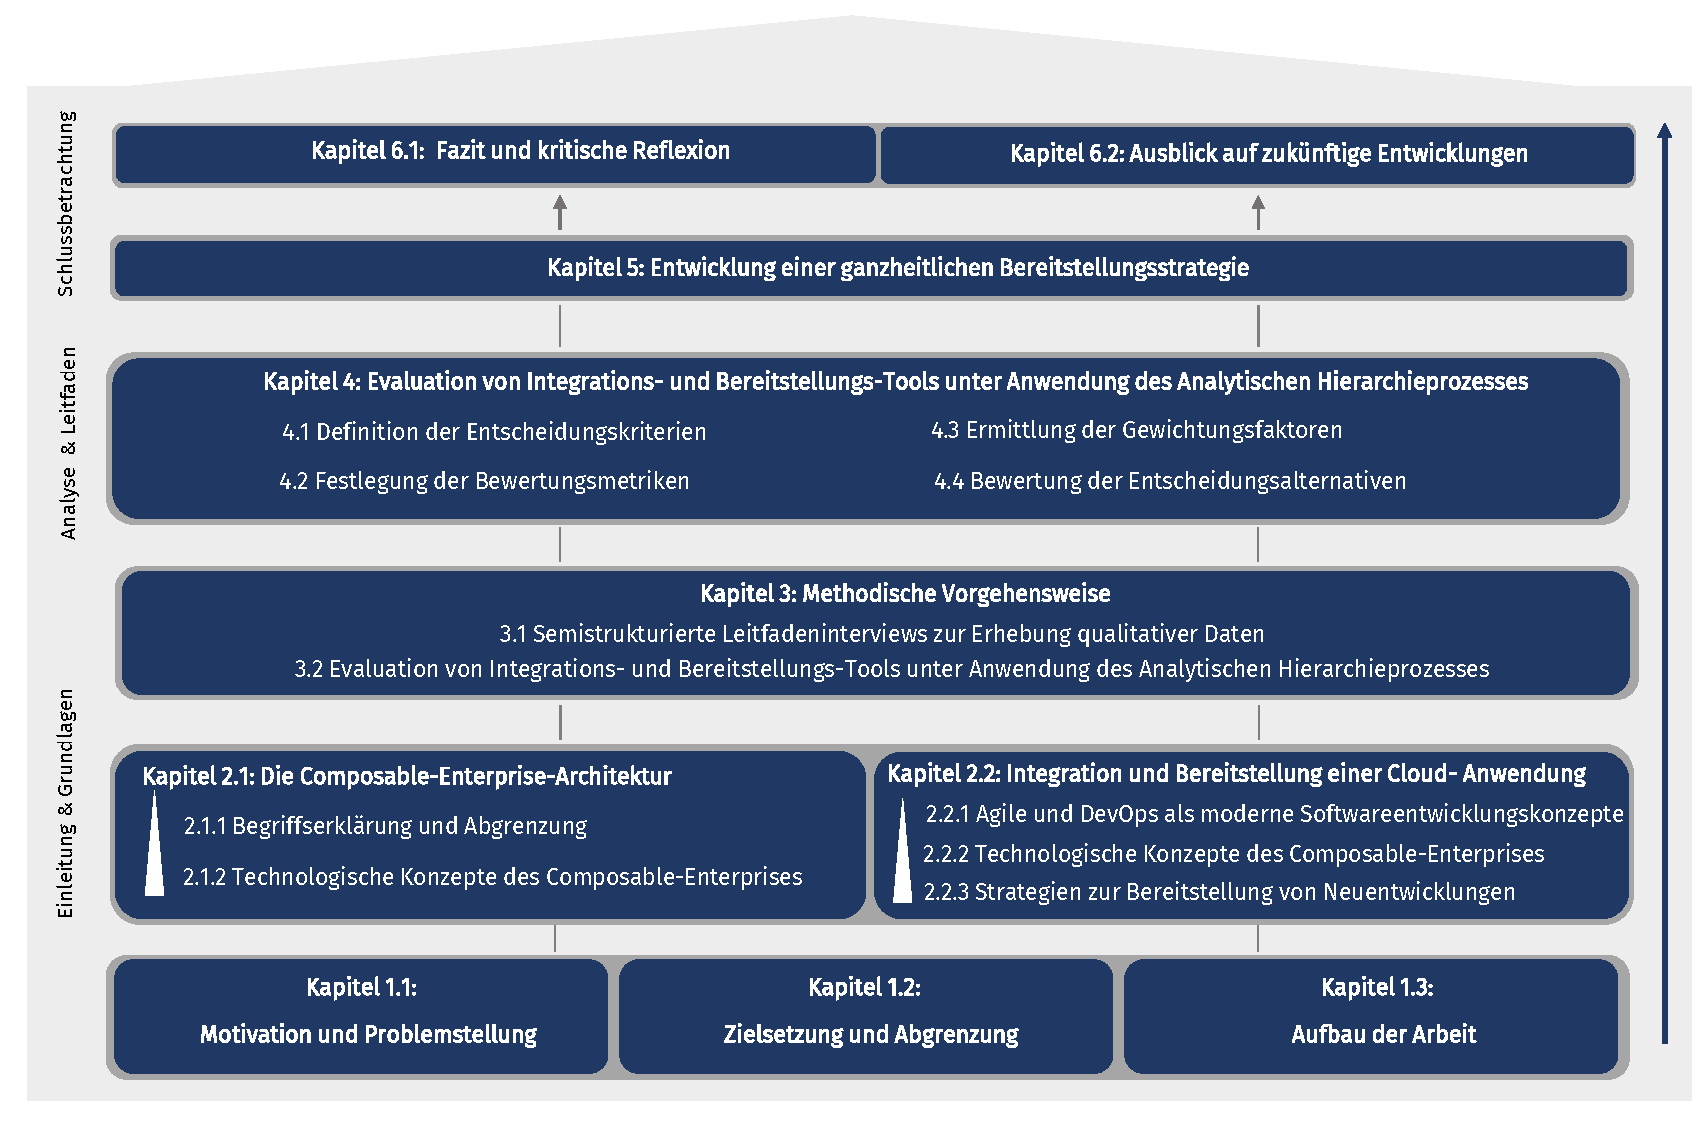
\includegraphics{Aufbau}}
		\caption[Aufbau der Arbeit]{Aufbau der Arbeit. Eigene Darstellung.}
		\label{fig:Aufbau}
	\end{figure}	
\end{center}
\vspace*{-15mm}
